\documentclass[]{article}
\usepackage{lmodern}
\usepackage{amssymb,amsmath}
\usepackage{ifxetex,ifluatex}
\usepackage{fixltx2e} % provides \textsubscript
\ifnum 0\ifxetex 1\fi\ifluatex 1\fi=0 % if pdftex
  \usepackage[T1]{fontenc}
  \usepackage[utf8]{inputenc}
\else % if luatex or xelatex
  \ifxetex
    \usepackage{mathspec}
  \else
    \usepackage{fontspec}
  \fi
  \defaultfontfeatures{Ligatures=TeX,Scale=MatchLowercase}
\fi
% use upquote if available, for straight quotes in verbatim environments
\IfFileExists{upquote.sty}{\usepackage{upquote}}{}
% use microtype if available
\IfFileExists{microtype.sty}{%
\usepackage{microtype}
\UseMicrotypeSet[protrusion]{basicmath} % disable protrusion for tt fonts
}{}
\usepackage[margin=1in]{geometry}
\usepackage{hyperref}
\hypersetup{unicode=true,
            pdftitle={Compulsory exercise 2: Group XX},
            pdfauthor={NN1, NN2 and NN3},
            pdfborder={0 0 0},
            breaklinks=true}
\urlstyle{same}  % don't use monospace font for urls
\usepackage{color}
\usepackage{fancyvrb}
\newcommand{\VerbBar}{|}
\newcommand{\VERB}{\Verb[commandchars=\\\{\}]}
\DefineVerbatimEnvironment{Highlighting}{Verbatim}{commandchars=\\\{\}}
% Add ',fontsize=\small' for more characters per line
\usepackage{framed}
\definecolor{shadecolor}{RGB}{248,248,248}
\newenvironment{Shaded}{\begin{snugshade}}{\end{snugshade}}
\newcommand{\KeywordTok}[1]{\textcolor[rgb]{0.13,0.29,0.53}{\textbf{#1}}}
\newcommand{\DataTypeTok}[1]{\textcolor[rgb]{0.13,0.29,0.53}{#1}}
\newcommand{\DecValTok}[1]{\textcolor[rgb]{0.00,0.00,0.81}{#1}}
\newcommand{\BaseNTok}[1]{\textcolor[rgb]{0.00,0.00,0.81}{#1}}
\newcommand{\FloatTok}[1]{\textcolor[rgb]{0.00,0.00,0.81}{#1}}
\newcommand{\ConstantTok}[1]{\textcolor[rgb]{0.00,0.00,0.00}{#1}}
\newcommand{\CharTok}[1]{\textcolor[rgb]{0.31,0.60,0.02}{#1}}
\newcommand{\SpecialCharTok}[1]{\textcolor[rgb]{0.00,0.00,0.00}{#1}}
\newcommand{\StringTok}[1]{\textcolor[rgb]{0.31,0.60,0.02}{#1}}
\newcommand{\VerbatimStringTok}[1]{\textcolor[rgb]{0.31,0.60,0.02}{#1}}
\newcommand{\SpecialStringTok}[1]{\textcolor[rgb]{0.31,0.60,0.02}{#1}}
\newcommand{\ImportTok}[1]{#1}
\newcommand{\CommentTok}[1]{\textcolor[rgb]{0.56,0.35,0.01}{\textit{#1}}}
\newcommand{\DocumentationTok}[1]{\textcolor[rgb]{0.56,0.35,0.01}{\textbf{\textit{#1}}}}
\newcommand{\AnnotationTok}[1]{\textcolor[rgb]{0.56,0.35,0.01}{\textbf{\textit{#1}}}}
\newcommand{\CommentVarTok}[1]{\textcolor[rgb]{0.56,0.35,0.01}{\textbf{\textit{#1}}}}
\newcommand{\OtherTok}[1]{\textcolor[rgb]{0.56,0.35,0.01}{#1}}
\newcommand{\FunctionTok}[1]{\textcolor[rgb]{0.00,0.00,0.00}{#1}}
\newcommand{\VariableTok}[1]{\textcolor[rgb]{0.00,0.00,0.00}{#1}}
\newcommand{\ControlFlowTok}[1]{\textcolor[rgb]{0.13,0.29,0.53}{\textbf{#1}}}
\newcommand{\OperatorTok}[1]{\textcolor[rgb]{0.81,0.36,0.00}{\textbf{#1}}}
\newcommand{\BuiltInTok}[1]{#1}
\newcommand{\ExtensionTok}[1]{#1}
\newcommand{\PreprocessorTok}[1]{\textcolor[rgb]{0.56,0.35,0.01}{\textit{#1}}}
\newcommand{\AttributeTok}[1]{\textcolor[rgb]{0.77,0.63,0.00}{#1}}
\newcommand{\RegionMarkerTok}[1]{#1}
\newcommand{\InformationTok}[1]{\textcolor[rgb]{0.56,0.35,0.01}{\textbf{\textit{#1}}}}
\newcommand{\WarningTok}[1]{\textcolor[rgb]{0.56,0.35,0.01}{\textbf{\textit{#1}}}}
\newcommand{\AlertTok}[1]{\textcolor[rgb]{0.94,0.16,0.16}{#1}}
\newcommand{\ErrorTok}[1]{\textcolor[rgb]{0.64,0.00,0.00}{\textbf{#1}}}
\newcommand{\NormalTok}[1]{#1}
\usepackage{graphicx,grffile}
\makeatletter
\def\maxwidth{\ifdim\Gin@nat@width>\linewidth\linewidth\else\Gin@nat@width\fi}
\def\maxheight{\ifdim\Gin@nat@height>\textheight\textheight\else\Gin@nat@height\fi}
\makeatother
% Scale images if necessary, so that they will not overflow the page
% margins by default, and it is still possible to overwrite the defaults
% using explicit options in \includegraphics[width, height, ...]{}
\setkeys{Gin}{width=\maxwidth,height=\maxheight,keepaspectratio}
\IfFileExists{parskip.sty}{%
\usepackage{parskip}
}{% else
\setlength{\parindent}{0pt}
\setlength{\parskip}{6pt plus 2pt minus 1pt}
}
\setlength{\emergencystretch}{3em}  % prevent overfull lines
\providecommand{\tightlist}{%
  \setlength{\itemsep}{0pt}\setlength{\parskip}{0pt}}
\setcounter{secnumdepth}{0}
% Redefines (sub)paragraphs to behave more like sections
\ifx\paragraph\undefined\else
\let\oldparagraph\paragraph
\renewcommand{\paragraph}[1]{\oldparagraph{#1}\mbox{}}
\fi
\ifx\subparagraph\undefined\else
\let\oldsubparagraph\subparagraph
\renewcommand{\subparagraph}[1]{\oldsubparagraph{#1}\mbox{}}
\fi

%%% Use protect on footnotes to avoid problems with footnotes in titles
\let\rmarkdownfootnote\footnote%
\def\footnote{\protect\rmarkdownfootnote}

%%% Change title format to be more compact
\usepackage{titling}

% Create subtitle command for use in maketitle
\newcommand{\subtitle}[1]{
  \posttitle{
    \begin{center}\large#1\end{center}
    }
}

\setlength{\droptitle}{-2em}
  \title{Compulsory exercise 2: Group XX}
  \pretitle{\vspace{\droptitle}\centering\huge}
  \posttitle{\par}
\subtitle{TMA4268 Statistical Learning V2018}
  \author{NN1, NN2 and NN3}
  \preauthor{\centering\large\emph}
  \postauthor{\par}
  \predate{\centering\large\emph}
  \postdate{\par}
  \date{14 mars, 2018}


\begin{document}
\maketitle

\subsection{1a)}\label{a}

\begin{itemize}
\item
  Q1: We have \(d\) possible predictors. For each predictor, we can
  either use it, or we can not use it. Hence we have two unique
  possibilities in \(d\) variables, resulting in a total of \(2^d\)
  possible combinations. Thus, the number of different regression models
  is given by \(2^d\). Another way to see this is by investigating each
  model complexity independently. Say we use \(k\) predictors in our
  model. We then choose \(k\) different predictors from \(d\) possible
  ones, and we can not choose the same twice. Hence, the number of
  possible combinations using \(k\) predictors is given by the standard
  nCr-formula \(\binom{d}{k}\). Now we have our \(d\) different choices
  of \(k\), which all gives different linear regression models. In
  total, the number of models is
  \[\binom{d}{0}+\binom{d}{1}+\dots+\binom{d}{d}.\] The binomial theorem
  states that \[(1+x)^n=\sum_{k=0}^n \binom{n}{k} x^k.\]. By setting
  \(x=1\), we see that the number of different linear regression models
  is given by \[\sum_{k=1}^d \binom{d}{k}=2^d.\]
\item
  Q2: The following algorithm illustrates how the best subset method
  finds the best model amongst the \(2^d\) possible ones: Denote first
  by \(\mathcal{M}_0\) the model using no predictors. This model simply
  predicts the sample mean for new observations. Next, for
  \(k=1,2,\dots,d\), fit all \(\binom{d}{k}\) models, by solving the
  equation
  \(\hat{\boldsymbol \beta} =(\boldsymbol X^T \boldsymbol X)^{-1} \boldsymbol X^T \boldsymbol Y\),
  where \(\boldsymbol{X}\) and \(\boldsymbol{Y}\) only contains the
  predictors for one specific model. Calculate the RSS, and choose the
  model with the lowest RSS amongst the \(\binom{d}{k}\) models, to be
  considered later. Now after the for-loop, we have \(d+1\) possible
  models to consider. Calculate
  \(BIC=\frac{1}{n}(RSS+log(n)k\hat \sigma^2)\) for each, where
  \(\hat \sigma^2\) is a unbiased estimator for the variance, and choose
  the model with the lowest \(BIC\). This is the best model by the best
  subset method, using \(BIC\)-criterion. \(R^2\) is given by
  \(1-RSS/TSS\). In this expression, we do not care how many predictors
  are being used. This is a problem, because training error is a poor
  estimate for test error, since it may cause overfitting. A possible
  solution to this is to add penalties, depending on how many predictors
  we use. If we were to use \(R^2\) instead of \(BIC\) to choose the
  best model, our best model would surely contain all \(d\) predictors
  since over-fitting would make our model fit the training data better.
  This is unwanted as we would rather have a model that best fit test
  data, which \(BIC\) better simulates.
  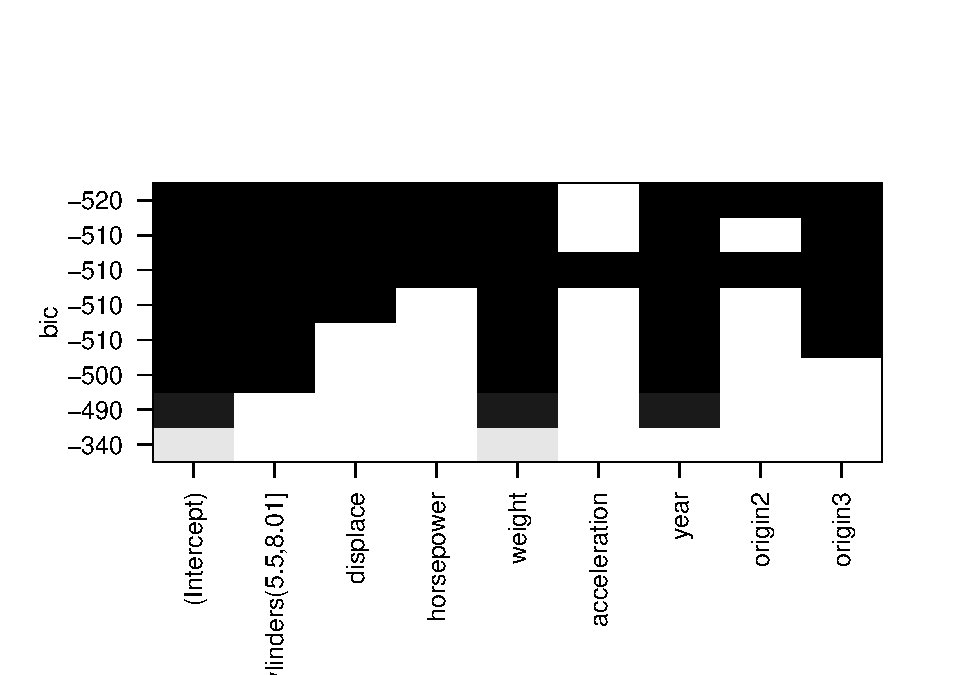
\includegraphics{Project2_files/figure-latex/unnamed-chunk-1-1.pdf}
\end{itemize}

\subsection{1b)}\label{b}

\begin{itemize}
\item
  Q3: As explained in Q2, \(RSS\) is calculated for all models, and for
  each model complexity, we choose the model with the lowest \(RSS\) as
  our best model. The \texttt{regsubsets}-function in R performs the
  actual calculations, and in the summary we can see which predictors
  corresponds to the lowest \(RSS\) for each model complexity. We see
  from this summary, which is printed in the task, that the best model
  with two predictors uses the ``weight'' and ``year'' columns, in
  addition to the intercept.
\item
  Q4: Now assuming we have the best model for each model complexity, we
  still want to choose which model complexity to use. As discussed in
  Q2, we expect to have the smallest \(RSS\) for the highest possible
  model complexity in the training set, but since we want to avoid
  overfitting, we add penalties to more complex models. Therefore, for
  each model complexity, we add the penalties according to the
  \(BIC\)-criterion, and then choose the model with the lowest value as
  our best method. The \(regsubsets\)-function in R also does the
  calculations for the penalties, using \(BIC\)-criterion in addition to
  other penalty-adding methods. Thus we can from the
  \texttt{regsubsets}-function also retrieve the \(BIC\)-values for each
  model complexity, and choose the lowest one as our model. The figure
  above, which is the result of plotting the \texttt{regsubsets}-data
  also contains the necessary information for choosing the best model.
  On the \(y\) scale, we see \(BIC\)-values for the models of different
  complexity, and on the \(x\)-scale we see which predictors are
  contained in the best model of this complexity, as a black box. We
  choose the model with the lowest \(BIC\)-value, which we see has
  \(BIC\approx -520\), and contains seven predictors, all but
  acceleration. Hence, this is our best model according to the best
  subset method using \(BIC\)-criterion on the training data. From the
  prints in the task we see the more exact value \(BIC=-516.9417\),
  which was rounded off to -520. The following R-code fits this model to
  the training data, by using the \texttt{lm}-function. The summary
  output gives us information about how well the model fit. We see that
  all of the \(t\)-values are fairly high, and the \(p\)-values for all
  but one are within the 0.001-significance level, while the last one is
  within the 0.01 significance level. It is therefore reasonable to
  assume there is a linear connection between miles per gallon and the
  other variates. We also see R-squared-values relatively close to 1,
  which indicates a good model fit. We have \(RSS=RSE^2(n-k-1)\), so
  that
  \[MSE=\frac{RSS}{n}=\frac{RSE^2(n-k-1)}{n}=\frac{3.233^2\cdot 305}{313}=10.185.\]
  The train-\(MSE\) is also calculated in the code below, giving the
  result 10.184, which is different probably because of roundoff-error.
  We have also performed an Anderson-Darling test for Normality. The
  \(p\)-value for this test is \(9.241\cdot 10^{-6}\), which is very
  small, and indicates that our data does not have normal distributed
  errors. ???
\end{itemize}

\begin{Shaded}
\begin{Highlighting}[]
\KeywordTok{library}\NormalTok{(nortest)}
\NormalTok{trainLm=}\KeywordTok{lm}\NormalTok{(mpg}\OperatorTok{~}\NormalTok{. }\OperatorTok{-}\NormalTok{acceleration, }\DataTypeTok{data=}\NormalTok{ourAutoTrain)}
\KeywordTok{summary}\NormalTok{(trainLm)}
\KeywordTok{ad.test}\NormalTok{(}\KeywordTok{rstudent}\NormalTok{(trainLm))}
\NormalTok{yhat_train=}\KeywordTok{predict}\NormalTok{(trainLm,ourAutoTrain)}
\NormalTok{yhat_test=}\KeywordTok{predict}\NormalTok{(trainLm,ourAutoTest)}
\NormalTok{MSE_train=}\KeywordTok{mean}\NormalTok{((ourAutoTrain}\OperatorTok{$}\NormalTok{mpg}\OperatorTok{-}\NormalTok{yhat_train)}\OperatorTok{^}\DecValTok{2}\NormalTok{)}
\NormalTok{MSE_train}
\NormalTok{MSE_test=}\KeywordTok{mean}\NormalTok{((ourAutoTest}\OperatorTok{$}\NormalTok{mpg}\OperatorTok{-}\NormalTok{yhat_test)}\OperatorTok{^}\DecValTok{2}\NormalTok{)}
\NormalTok{MSE_test}
\end{Highlighting}
\end{Shaded}

\begin{verbatim}
## 
## Call:
## lm(formula = mpg ~ . - acceleration, data = ourAutoTrain)
## 
## Residuals:
##     Min      1Q  Median      3Q     Max 
## -8.7254 -2.0561 -0.3412  1.7122 12.9550 
## 
## Coefficients:
##                       Estimate Std. Error t value Pr(>|t|)    
## (Intercept)         -1.941e+01  4.589e+00  -4.230 3.09e-05 ***
## cylinders(5.5,8.01] -3.533e+00  7.469e-01  -4.730 3.43e-06 ***
## displace             3.279e-02  6.749e-03   4.858 1.90e-06 ***
## horsepower          -4.883e-02  1.184e-02  -4.124 4.80e-05 ***
## weight              -5.824e-03  6.185e-04  -9.415  < 2e-16 ***
## year                 7.849e-01  5.699e-02  13.771  < 2e-16 ***
## origin2              1.794e+00  6.204e-01   2.892  0.00411 ** 
## origin3              2.906e+00  5.943e-01   4.891 1.63e-06 ***
## ---
## Signif. codes:  0 '***' 0.001 '**' 0.01 '*' 0.05 '.' 0.1 ' ' 1
## 
## Residual standard error: 3.233 on 305 degrees of freedom
## Multiple R-squared:  0.8344, Adjusted R-squared:  0.8306 
## F-statistic: 219.6 on 7 and 305 DF,  p-value: < 2.2e-16
## 
## 
##  Anderson-Darling normality test
## 
## data:  rstudent(trainLm)
## A = 2.2684, p-value = 9.241e-06
## 
## [1] 10.18351
## [1] 8.931018
\end{verbatim}

\begin{itemize}
\tightlist
\item
  Q5: The code above also predicts new values for the test set, and
  calculates the test-\(MSE\). Here, we got \(MSE=8.931\), which
  actually is smaller than the training \(MSE\), indicating that we
  indeed have managed to avoid overfitting, and made a model which
  predicts new values pretty well.
\end{itemize}

\subsection{1c)}\label{c}

\begin{itemize}
\item
  Q6. K-fold cross-validation involves dividing the data into \(k\)
  folds, \(C_1, C_2, \dots, C_k\). We then want to divide the data into
  a training and test set, and we choose one of the \(k\) parts as the
  test set, while we let the rest be training data. After fitting the
  model, we calculate \(MSE\) for the specific test folder, as
  \[MSE_j=\frac{1}{n_k}\sum_{i \in C_j}(y_i-\hat y_i)^2,\] where
  \(n_k=n/k\). Furthermore, we want to use all the folds as testing data
  in turn, while we let the \(k-1\) remaining folds be training data to
  fit different models. Thus, we calculate
  \(MSE_1, MSE_2,\dots, MSE_k\), and finally we give the
  cross-validation a value as \[CV_k=\frac{n_k}{n}\sum_{j=1}^k MSE_j.\]
  In our regression setting, when doing this for different complexities,
  we want to find which complexity gives the lowest \(CV_k\), and we
  choose this as our best model.
\item
  Q7. LOOCV suffers from quite high variance, since the training sets
  only differ with one observation. This makes the training sets have a
  very high correlation, and we choose our model based on an average of
  these corrolated models. This, in the end, can give a high variance.
  By using k-fold cross-validation instead we can lower the variance.
  Note however that this is at the cost of a higher bias, since the
  dataset used for fitting the models are smaller by a factor of
  \((k-1)/k\). k-fold cross-valudation with \(k=5\) or \(k=10\) is often
  seen as a compromise between the high variance and the high bias. In
  addition, it is more expensive to implement LOOVC, since you have to
  fit \(n\) data sets, instead of \(k\), resulting in more calculations.
  It is thus less work using k-fold cross-validation.
\end{itemize}

\subsection{1d}\label{d}

\begin{itemize}
\tightlist
\item
  Q8. The R-code for performing 10-fold cross validation is below.
\end{itemize}

\begin{Shaded}
\begin{Highlighting}[]
\KeywordTok{library}\NormalTok{(caret)}
\KeywordTok{library}\NormalTok{(leaps)}
\NormalTok{predict.regsubsets=}\ControlFlowTok{function}\NormalTok{(object,newdata,id)\{}
\NormalTok{  form=}\KeywordTok{as.formula}\NormalTok{(object}\OperatorTok{$}\NormalTok{call[[}\DecValTok{2}\NormalTok{]])}
\NormalTok{  mat=}\KeywordTok{model.matrix}\NormalTok{(form,newdata)}
\NormalTok{  coefi=}\KeywordTok{coef}\NormalTok{(object,}\DataTypeTok{id=}\NormalTok{id)}
\NormalTok{  xvars=}\KeywordTok{names}\NormalTok{(coefi)}
\NormalTok{  mat[,xvars]}\OperatorTok\NormalTok{coefi}
\NormalTok{\}}
\NormalTok{k=}\DecValTok{10}
\KeywordTok{set.seed}\NormalTok{(}\DecValTok{4268}\NormalTok{)}
\NormalTok{folds=}\KeywordTok{sample}\NormalTok{(}\DecValTok{1}\OperatorTok{:}\NormalTok{k,}\KeywordTok{nrow}\NormalTok{(ourAutoTrain),}\DataTypeTok{replace=}\OtherTok{TRUE}\NormalTok{)}
\NormalTok{cv.errors=}\KeywordTok{matrix}\NormalTok{(}\OtherTok{NA}\NormalTok{,k,}\DecValTok{8}\NormalTok{,}\DataTypeTok{dimnames=}\KeywordTok{list}\NormalTok{(}\OtherTok{NULL}\NormalTok{,}\KeywordTok{paste}\NormalTok{(}\DecValTok{1}\OperatorTok{:}\DecValTok{8}\NormalTok{)))}
\ControlFlowTok{for}\NormalTok{ (j }\ControlFlowTok{in} \DecValTok{1}\OperatorTok{:}\NormalTok{k)\{}
\NormalTok{  best.fit=}\KeywordTok{regsubsets}\NormalTok{(mpg}\OperatorTok{~}\NormalTok{.,}\DataTypeTok{data=}\NormalTok{ourAutoTrain[folds}\OperatorTok{!=}\NormalTok{j,])}
  \ControlFlowTok{for}\NormalTok{ (i }\ControlFlowTok{in} \DecValTok{1}\OperatorTok{:}\DecValTok{8}\NormalTok{)\{}
\NormalTok{    pred=}\KeywordTok{predict.regsubsets}\NormalTok{(best.fit,ourAutoTrain[folds}\OperatorTok{==}\NormalTok{j,],}\DataTypeTok{id=}\NormalTok{i)}
\NormalTok{    cv.errors[j,i]=}\KeywordTok{mean}\NormalTok{((ourAutoTrain}\OperatorTok{$}\NormalTok{mpg[folds}\OperatorTok{==}\NormalTok{j]}\OperatorTok{-}\NormalTok{pred)}\OperatorTok{^}\DecValTok{2}\NormalTok{)}
\NormalTok{  \}}
\NormalTok{\}}
\NormalTok{mean.cv.errors=}\KeywordTok{apply}\NormalTok{(cv.errors,}\DecValTok{2}\NormalTok{,mean)}
\NormalTok{mean.cv.errors}
\KeywordTok{which.min}\NormalTok{(mean.cv.errors)}
\end{Highlighting}
\end{Shaded}

\begin{verbatim}
##        1        2        3        4        5        6        7        8 
## 20.04605 11.98844 11.92601 11.29254 11.71515 10.72818 10.56209 10.61032 
## 7 
## 7
\end{verbatim}

\begin{itemize}
\item
  Q9. We see from the output of the code the \(MSE\) for the different
  complexities, and we also see we get the lowest \(MSE\) when using
  seven predictors. Hence, we want to use the same model complexity as
  we did for the \(BIC\)-criterion.
\item
  Q10. Now that we have established which model complexity we want to
  use, we would like to fit this on our entire training set, to get the
  best model possible. We would therefore use the
  \texttt{regsubsets}-function on the training set, and choose the model
  using seven predictors. We do however note that this will give us the
  exact same model as we did for the \(BIC\)-criterion. Our comments on
  the model fit for the training set, and the \(MSE\) for the training
  set, is therefore identical to our results in Q4. Also, our predicted
  new values for the test set, and the MSE for the test set, is
  identical to our results in Q5. We therefore refer to Q4 and Q5 in
  this task.
\end{itemize}

\subsection{2a) Explain figures}\label{a-explain-figures}

\begin{itemize}
\item
  Q11. \(\lambda\) is a parameter which draws the estimated
  coeffiecients towards zero in both ridge and lasso regression. For
  very large \(\lambda\)'s, all the estimated coefficients are
  essentially zero. However, in ridge regression, none of the
  coefficients will be set exactly to zero. In comparison , the penalty
  term in lasso regression may set some of the coefficient to be exactly
  zero when \(\lambda\) is large enough. In Figure 1, we can see that
  this is the case, while the coefficients in Figure 2 do not seem to be
  exactly zero for any value of \(\lambda\) in the given interval. Thus,
  Figure 1 corresponds to lasso regression while Figure 2 corresponds to
  ridge regression.
\item
  Q12. As stated, we can see that the tuning parameter \(\lambda\) draws
  the \(\beta\)'s towards zero as \(\lambda\) increases. In lasso
  regression, all of the coefficients seem to become exactly zero, while
  in ridge regression, the coefficients are drawn towards zero, but are
  not exactly zero. When \(\lambda=0\), the penalty term in both ridge
  and lasso regression will disappear, so the coefficients will just be
  the same as with least squares estimation. At this value for
  \(\lambda\), the bias is zero, but the variance may be high. As
  \(\lambda\) increases, the variance will become lower as the
  coefficients are shrinked and flexibility decreases. However, the bias
  will increase at the same time. In both ridge and lasso regression,
  when \(\lambda \rightarrow \infty\), we have the null model, which
  means that all of the coefficient estimates are zero. Then the
  variance approaches zero, but the bias becomes large.
\item
  Q13. Ridge regression will include all \(p\) covariates, and thus can
  not be used to perform model selection. However, lasso regression can
  be used in the same way as best subset selection, as the variables are
  forced to be exactly zero when \(\lambda\) is large. For a given value
  of \(\lambda\), lasso regression may zero out some of the estimated
  coefficients and it thus performs a variable selection.
\end{itemize}

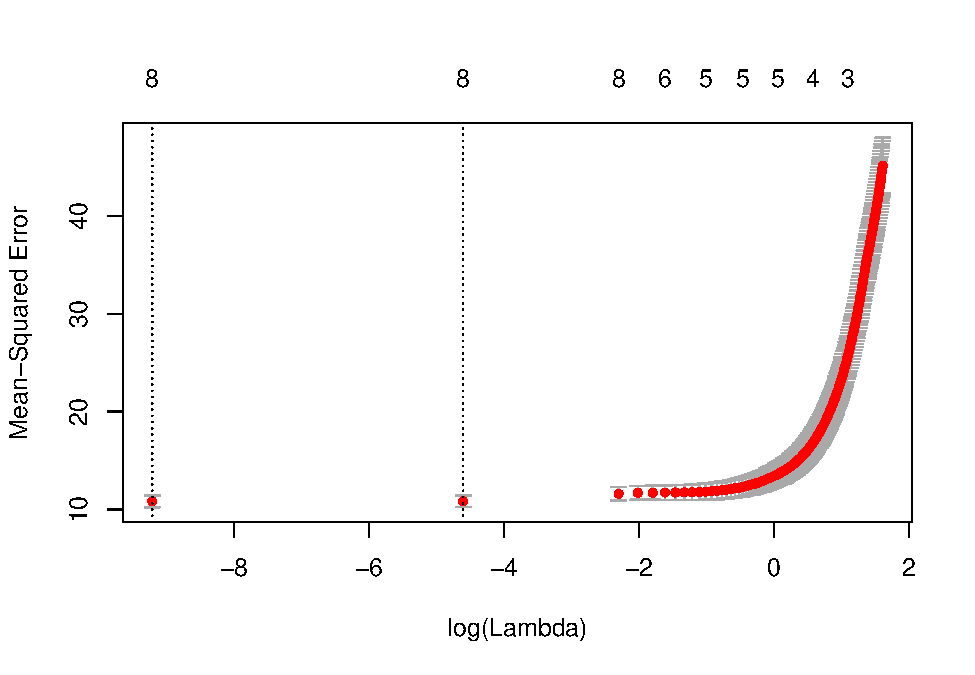
\includegraphics{Project2_files/figure-latex/unnamed-chunk-4-1.pdf}

\subsection{\texorpdfstring{2b) Finding the optimal
\(\lambda\)}{2b) Finding the optimal \textbackslash{}lambda}}\label{b-finding-the-optimal-lambda}

\begin{itemize}
\item
  Q14: The function cv.glmnet performs a k-fold cross-validation for a
  sequence of \(\lambda\)'s, produces a plot and returns an object with
  different ingredients.
\item
  Q15. The plot shows the cross-validation curve, including the upper
  and lower standard deviation curves along the sequence of
  \(\lambda\)'s. The \(\lambda\) with the lowest cross-validated MSE in
  the plot can be chosen as the optimal \(\lambda\):
\end{itemize}

\begin{Shaded}
\begin{Highlighting}[]
\NormalTok{cv.out}\OperatorTok{$}\NormalTok{lambda.min}
\end{Highlighting}
\end{Shaded}

\begin{verbatim}
## [1] 1e-04
\end{verbatim}

The \texttt{1se-rule}, is another way to choose which \(\lambda\) is
optimal. In the object returned by \texttt{cv.glmnet}, one of the values
is \texttt{lambda.1se}, which is the largest value of \(\lambda\) such
that the error is within one standard error of the minimum.

\begin{itemize}
\tightlist
\item
  Q16: By using the \texttt{1se-rule}, we get that the optimal
  \(\lambda\) is
\end{itemize}

\begin{Shaded}
\begin{Highlighting}[]
\NormalTok{cv.out}\OperatorTok{$}\NormalTok{lambda.1se}
\end{Highlighting}
\end{Shaded}

\begin{verbatim}
## [1] 0.01
\end{verbatim}

\subsection{2c) Prediction}\label{c-prediction}

\begin{itemize}
\tightlist
\item
  Q17: Using lasso regression with the optimal value of \(\lambda\)
  according to the \texttt{1se-rule}, \(\lambda=0.01\), we can fit the
  model. The coefficient estimates are
\end{itemize}

\begin{Shaded}
\begin{Highlighting}[]
\KeywordTok{coef}\NormalTok{(cv.out,}\DataTypeTok{s=}\StringTok{"lambda.1se"}\NormalTok{)}
\end{Highlighting}
\end{Shaded}

\begin{verbatim}
## 9 x 1 sparse Matrix of class "dgCMatrix"
##                                 1
## (Intercept)         -21.407540632
## cylinders(5.5,8.01]  -3.374630096
## displace              0.030954456
## horsepower           -0.035558382
## weight               -0.006071262
## acceleration          0.122203782
## year                  0.781813677
## origin2               1.675613651
## origin3               2.832358817
\end{verbatim}

Thus, we get the model fit
\(\hat{y}=-21.408-3.375x_{cylinders}+0.031x_{displace}-0.036x_{horsepower}-0.006x_{weight}+0.122x_{acceleration}+0.782x_{year}+1.676x_{origin2}+2.832x_{origin3}\).

\begin{itemize}
\tightlist
\item
  Q18: Using this model with optimal \(\lambda\) chosen according to the
  \texttt{1se-rule}, we can predict \texttt{mpg} for cars based on their
  data. For a car with 4 cylinders, \texttt{displace=150},
  \texttt{horsepower=100}, \texttt{weight=3000},
  \texttt{acceleration=10}, \texttt{year=82} and which comes from
  Europe, \texttt{mpg} is predicted as
\end{itemize}

\begin{Shaded}
\begin{Highlighting}[]
\KeywordTok{predict}\NormalTok{(cv.out, }\DataTypeTok{newx =}\KeywordTok{matrix}\NormalTok{(}\KeywordTok{c}\NormalTok{(}\DecValTok{0}\NormalTok{,}\DecValTok{150}\NormalTok{,}\DecValTok{100}\NormalTok{,}\DecValTok{3000}\NormalTok{,}\DecValTok{10}\NormalTok{,}\DecValTok{82}\NormalTok{,}\DecValTok{1}\NormalTok{,}\DecValTok{0}\NormalTok{),}\DataTypeTok{nrow=}\DecValTok{1}\NormalTok{), }\DataTypeTok{s =} \StringTok{"lambda.1se"}\NormalTok{)}
\end{Highlighting}
\end{Shaded}

\begin{verbatim}
##             1
## [1,] 28.47238
\end{verbatim}

\subsection{3a)}\label{a-1}

\begin{itemize}
\tightlist
\item
  Q19: Fitting the specified \texttt{gam}
\end{itemize}

\begin{Shaded}
\begin{Highlighting}[]
\KeywordTok{library}\NormalTok{(gam)}
\NormalTok{gamobject =}\StringTok{ }\KeywordTok{gam}\NormalTok{(mpg }\OperatorTok{~}\StringTok{ }\KeywordTok{bs}\NormalTok{(displace, }\DataTypeTok{knots  =} \DecValTok{290}\NormalTok{) }\OperatorTok{+}\StringTok{ }\KeywordTok{poly}\NormalTok{(horsepower, }\DecValTok{2}\NormalTok{)  }\OperatorTok{+}\StringTok{ }\NormalTok{weight }\OperatorTok{+}\StringTok{ }\KeywordTok{s}\NormalTok{(acceleration, }\DecValTok{3}\NormalTok{) }\OperatorTok{+}\StringTok{ }\KeywordTok{factor}\NormalTok{(origin),}\DataTypeTok{data=}\NormalTok{ourAutoTrain)}
\KeywordTok{par}\NormalTok{(}\DataTypeTok{mfrow=}\KeywordTok{c}\NormalTok{(}\DecValTok{2}\NormalTok{,}\DecValTok{3}\NormalTok{))}
\KeywordTok{plot}\NormalTok{(gamobject,}\DataTypeTok{se=}\OtherTok{TRUE}\NormalTok{,}\DataTypeTok{col=}\StringTok{"blue"}\NormalTok{)}
\NormalTok{M =}\StringTok{ }\DecValTok{4}
\NormalTok{cp =}\StringTok{ }\KeywordTok{c}\NormalTok{(}\DecValTok{290}\NormalTok{)}
\NormalTok{l =}\StringTok{ }\KeywordTok{c}\NormalTok{(}\DecValTok{0}\NormalTok{,}\DecValTok{500}\NormalTok{)}
\KeywordTok{par}\NormalTok{(}\DataTypeTok{mfrow =} \KeywordTok{c}\NormalTok{(}\DecValTok{2}\NormalTok{,}\DecValTok{2}\NormalTok{), }\DataTypeTok{mar =} \KeywordTok{c}\NormalTok{(}\DecValTok{2}\NormalTok{,}\DecValTok{2}\NormalTok{,}\DecValTok{2}\NormalTok{,}\DecValTok{2}\NormalTok{))}
\end{Highlighting}
\end{Shaded}

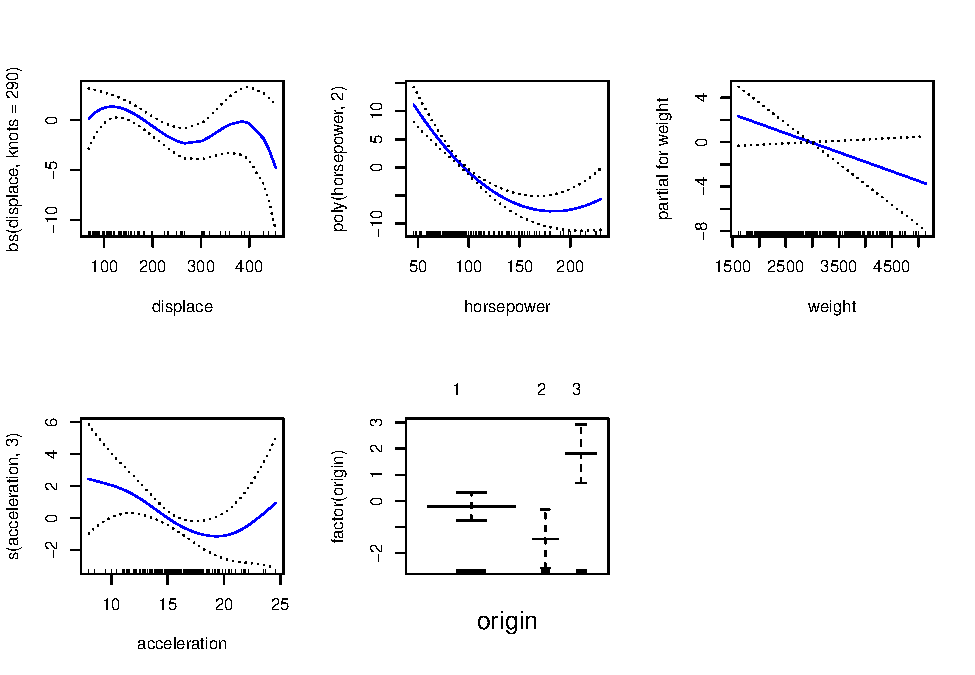
\includegraphics{Project2_files/figure-latex/unnamed-chunk-9-1.pdf}

\begin{Shaded}
\begin{Highlighting}[]
\NormalTok{s=}\KeywordTok{sapply}\NormalTok{(}\DecValTok{1}\OperatorTok{:}\NormalTok{(M}\OperatorTok{-}\DecValTok{1}\NormalTok{), }\ControlFlowTok{function}\NormalTok{(y) }\KeywordTok{curve}\NormalTok{(x}\OperatorTok{^}\NormalTok{y, l[}\DecValTok{1}\NormalTok{], l[}\DecValTok{2}\NormalTok{], }\DataTypeTok{yaxt =} \StringTok{"n"}\NormalTok{,}
 \DataTypeTok{ylab =} \StringTok{""}\NormalTok{, }\DataTypeTok{xlab =} \StringTok{""}\NormalTok{, }\DataTypeTok{main =} \KeywordTok{bquote}\NormalTok{(b[.(y)](x) }\OperatorTok{==}\StringTok{ }\NormalTok{x}\OperatorTok{^}\NormalTok{.(y))))}
\NormalTok{s=}\KeywordTok{sapply}\NormalTok{(}\DecValTok{1}\OperatorTok{:}\KeywordTok{length}\NormalTok{(cp), }\ControlFlowTok{function}\NormalTok{(y) }\KeywordTok{curve}\NormalTok{(}\KeywordTok{pmax}\NormalTok{(}\DecValTok{0}\NormalTok{,x}\OperatorTok{-}\NormalTok{cp[y])}\OperatorTok{^}\DecValTok{3}\NormalTok{, l[}\DecValTok{1}\NormalTok{], l[}\DecValTok{2}\NormalTok{], }\DataTypeTok{yaxt =} \StringTok{"n"}\NormalTok{,}
 \DataTypeTok{ylab =} \StringTok{""}\NormalTok{, }\DataTypeTok{xlab =} \StringTok{"displacement"}\NormalTok{, }\DataTypeTok{main =} \KeywordTok{bquote}\NormalTok{(b[.(y}\OperatorTok{+}\NormalTok{M}\OperatorTok{-}\DecValTok{1}\NormalTok{)](x) }\OperatorTok{==}\StringTok{ }\NormalTok{(x}\OperatorTok{-}\NormalTok{.(cp[y]))[}\StringTok{"+"}\NormalTok{]}\OperatorTok{^}\NormalTok{.(M}\OperatorTok{-}\DecValTok{1}\NormalTok{))))}
\end{Highlighting}
\end{Shaded}

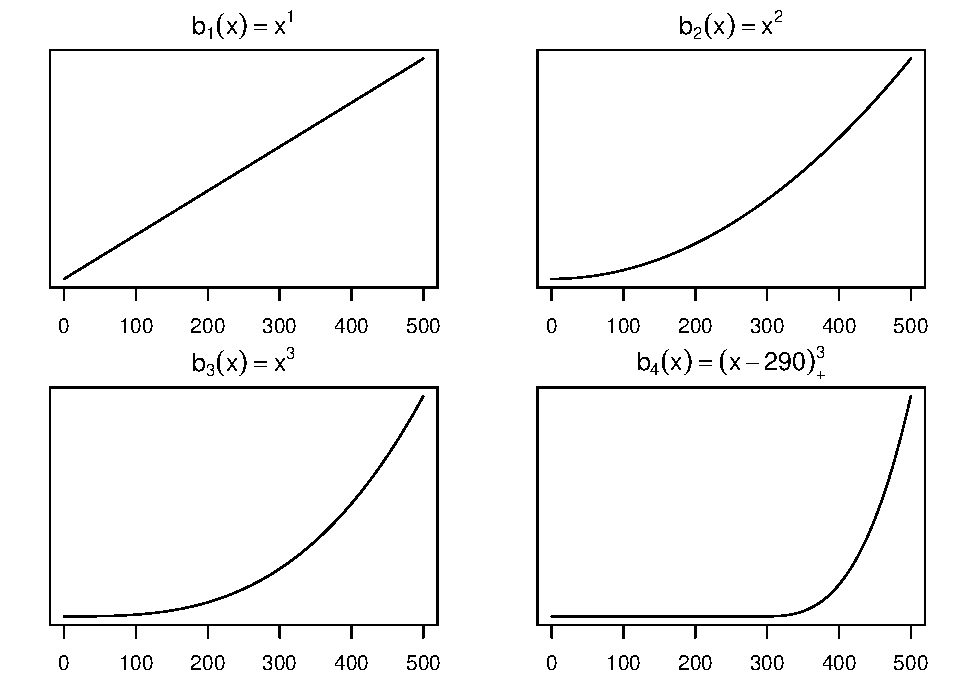
\includegraphics{Project2_files/figure-latex/unnamed-chunk-9-2.pdf}

\begin{itemize}
\tightlist
\item
  Q20: A basis for the cubic spline (displace) will be a combination of
  a step function at the knot and polynomials of degree, will be
  \(X, X^2, X^3, (X-290)^3_+\).
\end{itemize}


\end{document}
